\documentclass[DIN, pagenumber=false, fontsize=11pt, parskip=half]{scrartcl}

\usepackage[utf8]{inputenc}
\usepackage[T1]{fontenc}
\usepackage{template}
\usepackage{amsmath}
\usepackage{tikz}
\usetikzlibrary{arrows.meta}

\DeclareMathOperator{\lcm}{lcm}

\tikzset{
    relation/.style={
        dot/.style={circle, fill=black, inner sep=1.6pt},
        every path/.style={-{Stealth[length=2mm]}, semithick},
    },
}

\titlehead{\centering\small
    Worked solutions to selected exercises from\\
    Richard Hammack, \emph{Book of Proof, edition 2.2}\\
\rule{0.4\linewidth}{0.4pt}}

\title{}
\author{} % Oscar A. Carrera
\date{}

\begin{document}
\maketitle

\setcounter{section}{10}

\section{Relations}

\setcounter{subsection}{-1}
\subsection{Relations}

\begin{problems}
    \problem Let $A = \set{1,2,3,4,5,6}$. Write out the relation $R$ that expresses $|$ (divides) on $A$. Then illustrate it with a diagram.

    \answer
    \begin{align*}
        R &= \{ (1,1), (1,2), (1,3), (1,4), (1,5), (1,6), (2,2), (2,4), \\ 
          & \qquad (2,6), (3,3), (3,6), (4,4), (5,5), (6,6) \}
    \end{align*}

    \begin{center}
        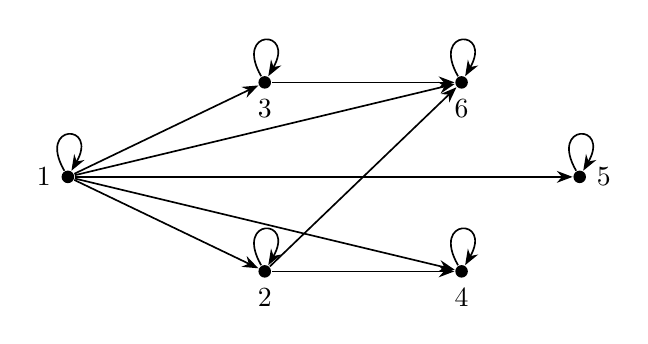
\begin{tikzpicture}[relation]
            \node[dot, label=left:$1$]  (1) at (0,0)      {};
            \node[dot, label=below:$2$] (2) at (2.5,-1.2) {};
            \node[dot, label=below:$3$] (3) at (2.5,1.2)  {};
            \node[dot, label=below:$4$] (4) at (5,-1.2)   {};
            \node[dot, label=right:$5$] (5) at (6.5,0)    {};
            \node[dot, label=below:$6$] (6) at (5,1.2)    {};
           
            \foreach \x in {1,...,6}
            \draw (\x) edge[loop above, min distance=7mm, in=60, out=120] (\x);
           
            \draw (1) -- (2);  \draw (1) -- (3);  \draw (1) -- (4);
            \draw (1) -- (5);  \draw (1) -- (6);
            \draw (2) -- (4);  \draw (2) -- (6);
            \draw (3) -- (6);
        \end{tikzpicture}
    \end{center}

    \problem[6] Congruence modulo 5 is a relation on the set $A = \mathbb{Z}$. In this relation $xRy$ means $x \equiv y \pmod{5}$. Write out the set $R$ in set-builder notation.

    \answer $R = \set{(x,y) \in \mathbb{Z} \times \mathbb{Z} : 5 \mid (x-y)}$.

    \problem Let $A = \set{1,2,3,4,5,6}$. Observe that $\emptyset \subseteq A \times A$, so $R = \emptyset$ is a relation on $A$. Draw a diagram for this relation.

    \answer Since $R = \emptyset$, no pair $(x,y)$ belongs to $R$, so the diagram has a node for each element of $A$ and no arrows at all.
    \begin{center}
        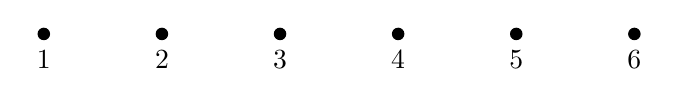
\begin{tikzpicture}[relation]
            \node[dot, label=below:$1$] (1) at (0,0)   {};
            \node[dot, label=below:$2$] (2) at (1.5,0) {};
            \node[dot, label=below:$3$] (3) at (3,0)   {};
            \node[dot, label=below:$4$] (4) at (4.5,0) {};
            \node[dot, label=below:$5$] (5) at (6,0)   {};
            \node[dot, label=below:$6$] (6) at (7.5,0) {};
        \end{tikzpicture}
    \end{center}

    \problem Consider the subset $R = (\mathbb{R} \times \mathbb{R}) - \set{(x,x) : x \in \mathbb{R}} \subseteq \mathbb{R} \times \mathbb{R}$. What familiar relation on $\mathbb{R}$ is this? Explain.

    \answer The relation is \textit{not equal ($\neq$)}. The set contains every pair $(x,y)$ of real numbers. Removing the pair $(x,x)$ leaves exactly the pairs where x and y differ. 
\end{problems}

\subsection{Properties of Relations}

\begin{problems}
    \problem Consider the relation $R = \set{(a,b),(a,c),(c,c),(b,b),(c,b),(b,c)}$ on the set $A = \set{a,b,c}$. Is $R$ reflexive? Symmetric? Transitive? If a property does not hold, say why.

    \answer This is not reflexive because $(a,a) \notin R$.\\ 
    This is not symmetric because $(a,b) \in R$ but $(b,a) \notin R$.\\ 
    This is transitive: checking every chain $xRy$, $yRz$ of pairs in $R$ confirms that $(x,z) \in R$ in each case.

    \problem Let $A = \set{a,b,c,d}$. Suppose $R$ is the relation
        \[
            \begin{aligned}
                R = \{ & (a,a),(b,b),(c,c),(d,d),(a,b),(b,a),(a,c),(c,a),\\
                       & (a,d),(d,a),(b,c),(c,b),(b,d),(d,b),(c,d),(d,c) \}.
            \end{aligned}
        \]
        Is $R$ reflexive? Symmetric? Transitive? If a property does not hold, say why.

    \answer This is reflexive because $xRx$ holds for every $x \in A$.\\ 
    This is symmetric because $xRy$ and $yRx$ both hold for every $x,y \in A$.\\ 
    This is transitive because $xRz$ holds for every $x,z \in A$, regardless of $y$.

    \problem Consider the relation $R = \set{(x,x) : x \in \mathbb{Z}}$ on $\mathbb{Z}$. Is $R$ reflexive? Symmetric? Transitive? If a property does not hold, say why. What familiar relation is this?

    \answer Here $xRy$ if and only if $x = y$, so $R$ is the equality relation $=$ on $\mathbb{Z}$.\\ 
    This is reflexive because $x = x$ for every $x \in \mathbb{Z}$.\\ 
    This is symmetric because $x = y$ implies $y = x$.\\ 
    This is transitive because $x = y$ and $y = z$ imply $x = z$.

    \problem Define a relation on $\mathbb{Z}$ as $xRy$ if $\abs{x-y} < 1$. Is $R$ reflexive? Symmetric? Transitive? If a property does not hold, say why. What familiar relation is this?

    \problem Suppose $A \neq \emptyset$. Since $\emptyset \subseteq A \times A$, the set $R = \emptyset$ is a relation on $A$. Is $R$ reflexive? Symmetric? Transitive? If a property does not hold, say why.

    \problem Prove that the relation $|$ (divides) on the set $\mathbb{Z}$ is reflexive and transitive. (Use Example 11.8 as a guide if you are unsure of how to proceed.)

    \problem Suppose $R$ is a symmetric and transitive relation on a set $A$, and there is an element $a \in A$ for which $aRx$ for every $x \in A$. Prove that $R$ is reflexive.

    \problem Define a relation $R$ on $\mathbb{Z}$ by declaring that $xRy$ if and only if $x^2 \equiv y^2 \pmod{4}$. Prove that $R$ is reflexive, symmetric and transitive.

    \problem The table on page 179 shows that relations on $\mathbb{Z}$ may obey various combinations of the reflexive, symmetric and transitive properties. In all, there are $2^3 = 8$ possible combinations, and the table shows 5 of them. (There is some redundancy, as $\leq$ and $|$ have the same type.) Complete the table by finding examples of relations on $\mathbb{Z}$ for the three missing combinations.
\end{problems}

\subsection{Equivalence Relations}

\begin{problems}
    \problem Let $A = \set{a,b,c,d,e}$. Suppose $R$ is an equivalence relation on $A$. Suppose $R$ has two equivalence classes. Also $aRd$, $bRc$ and $eRd$. Write out $R$ as a set.

    \problem Let $A = \set{a,b,c,d,e}$. Suppose $R$ is an equivalence relation on $A$. Suppose also that $aRd$ and $bRc$, $eRa$ and $cRe$. How many equivalence classes does $R$ have?

    \problem There are five different equivalence relations on the set $A = \set{a,b,c}$. Describe them all. Diagrams will suffice.

    \problem Define a relation $R$ on $\mathbb{Z}$ as $xRy$ if and only if $x^2 + y^2$ is even. Prove $R$ is an equivalence relation. Describe its equivalence classes.

    \problem Suppose $R$ and $S$ are two equivalence relations on a set $A$. Prove that $R \cap S$ is also an equivalence relation. (For an example of this, look at Figure 11.2. Observe that for the equivalence relations $R_2, R_3$ and $R_4$, we have $R_2 \cap R_3 = R_4$.)

    \problem Prove or disprove: If $R$ and $S$ are two equivalence relations on a set $A$, then $R \cup S$ is also an equivalence relation on $A$.

    \problem Suppose $R$ is a reflexive and symmetric relation on a finite set $A$. Define a relation $S$ on $A$ by declaring $xSy$ if and only if for some $n \in \mathbb{N}$ there are elements $x_1, x_2, \dots, x_n \in A$ satisfying $xRx_1$, $x_1Rx_2$, $x_2Rx_3$, $x_3Rx_4, \dots, x_{n-1}Rx_n$, and $x_nRy$. Show that $S$ is an equivalence relation and $R \subseteq S$. Prove that $S$ is the unique smallest equivalence relation on $A$ containing $R$.
\end{problems}

\subsection{Equivalence Classes and Partitions}

\begin{problems}
    \problem List all the partitions of the set $A = \set{a,b,c}$. Compare your answer to the answer to Exercise 6 of Section 11.2.

    \problem Suppose $P$ is a partition of a set $A$. Define a relation $R$ on $A$ by declaring $xRy$ if and only if $x,y \in X$ for some $X \in P$. Prove $R$ is an equivalence relation on $A$. Then prove that $P$ is the set of equivalence classes of $R$.
\end{problems}

\subsection{The Integers Modulo $n$}

\begin{problems}
    \problem Write the addition and multiplication tables for $\mathbb{Z}_3$.

    \problem Write the addition and multiplication tables for $\mathbb{Z}_6$.

    \problem Suppose $[a],[b] \in \mathbb{Z}_6$ and $[a] \cdot [b] = [0]$. Is it necessarily true that either $[a] = [0]$ or $[b] = [0]$?

    \problem Suppose $[a],[b] \in \mathbb{Z}_n$, and $[a] = [a']$ and $[b] = [b']$. Alice adds $[a]$ and $[b]$ as $[a]+[b] = [a+b]$. Bob adds them as $[a']+[b'] = [a'+b']$. Show that their answers $[a+b]$ and $[a'+b']$ are the same.
\end{problems}

\end{document}
